\documentclass{article}

% if you need to pass options to natbib, use, e.g.:
%     \PassOptionsToPackage{numbers, compress}{natbib}
% before loading neurips_2020

% ready for submission
% \usepackage{neurips_2020}

% to compile a preprint version, e.g., for submission to arXiv, add add the
% [preprint] option:
%     \usepackage[preprint]{neurips_2020}

% to compile a camera-ready version, add the [final] option, e.g.:
%     \usepackage[final]{neurips_2020}

% to avoid loading the natbib package, add option nonatbib:
     \usepackage[nonatbib]{neurips_2020}

\usepackage[utf8]{inputenc} % allow utf-8 input
\usepackage[T1]{fontenc}    % use 8-bit T1 fonts
\usepackage{hyperref}       % hyperlinks
\usepackage{url}            % simple URL typesetting
\usepackage{booktabs}       % professional-quality tables
\usepackage{amsfonts}       % blackboard math symbols
\usepackage{nicefrac}       % compact symbols for 1/2, etc.
\usepackage{microtype}      % microtypography
\usepackage[english]{babel}
\usepackage[utf8]{inputenc}
\usepackage{listings}
\usepackage{color}
\usepackage{algorithm}
\usepackage{algorithmic}
\usepackage{todonotes}
\usepackage{siunitx}
\usepackage{authblk}
\usepackage{subcaption}
\usepackage{bbm}
\usepackage{amsmath}

\graphicspath{ {.} }
\include{Commands}
\newtheorem{theorem}{Theorem}

\definecolor{dkgreen}{rgb}{0,0.6,0}
\definecolor{gray}{rgb}{0.5,0.5,0.5}
\definecolor{mauve}{rgb}{0.58,0,0.82}

\lstset{frame=tb,
	language=Java,
	aboveskip=3mm,
	belowskip=3mm,
	showstringspaces=false,
	columns=flexible,
	basicstyle={\small\ttfamily},
	numbers=none,
	numberstyle=\tiny\color{gray},
	keywordstyle=\color{blue},
	commentstyle=\color{dkgreen},
	stringstyle=\color{mauve},
	breaklines=true,
	breakatwhitespace=true,
	tabsize=3
}

\title{BitTensor: An Intermodel Intelligence Measure}

% The \author macro works with any number of authors. There are two commands
% used to separate the names and addresses of multiple authors: \And and \AND.
%
% Using \And between authors leaves it to LaTeX to determine where to break the
% lines. Using \AND forces a line break at that point. So, if LaTeX puts 3 of 4
% authors names on the first line, and the last on the second line, try using
% \AND instead of \And before the third author name.
  % examples of more authors
  % \And
  % Coauthor \\
  % Affiliation \\
  % Address \\
  % \texttt{email} \\
  % \AND
  % Coauthor \\
  % Affiliation \\
  % Address \\
  % \texttt{email} \\
  % \And
  % Coauthor \\
  % Affiliation \\
  % Address \\
  % \texttt{email} \\
  % \And
  % Coauthor \\
  % Affiliation \\
  % Address \\
  % \texttt{email} \\


\begin{document}

\maketitle

\begin{abstract}

The dominant approach to creating a machine learning system is to collect a dataset of training examples that demonstrate correct behavior for a desired task, then train that system to imitate these behaviors \cite{radford2019language}. Labeled datasets that evaluate the performance of intelligent systems on specific predefined tasks -- also known as benchmarks -- are the typical tools used to measure and reward the advancement of machine intelligence. We argue that a reward mechanism based on these tasks where progress is measured as test scores is low resolution, misaligned, and introduces wide-scale inefficiencies in developing machine learning systems. To reconcile these issues, we propose BitTensor: a benchmark where intelligence is measured by other intelligence systems rather than against task-based tests. We describe how this novel benchmark is constructed and how it is negotiated by computers that share knowledge peer-to-peer (P2P) across the internet. However since negotiation introduces game-theoretic considerations, we design methods to ensure veracity of the benchmark when peers remain self-interested and trustless. To test our design, we empirically show that the self-interested negotiation produces the desired ranking at the competitive equilibrium. The result is a benchmark which is simultaneously higher dimensional and divisible allows for a much larger and continually expanding definition of intelligence is inherently collaborative, open, decentralized, and can consume resources connected by an internet fabric. 

%%% OLD ABSTRACT
 %We argue that using labeled datasets creates single-subject matter experts that generalize rather poorly, with self-contained knowledge that cannot be shared with other models. To reconcile this, we propose BitTensor: a framework in which other models measure the informational significance of their peers across a network. Each model uses a digital ledger to negotiate their significance to the network. In doing so, BitTensor measures intelligence of each model with respect to intelligence itself, rather than via a projection onto labeled datasets. Additionally, we show how competition for connectivity in the network can be used to force honest bidding. We first prove that selecting inter-model scores using gradient descent is a regret-free strategy: one which generates the best subjective outcome regardless of the behavior of others. We then empirically show that when nodes apply this strategy, the network converges to a ranking that correlates with the one found in a fully coordinated and centralized setting. The result is a fair mechanism for training an internet-wide, decentralized and incentivized machine learning system. Such a system produces – on an ongoing basis – a continually hardening and expanding benchmark at the generalized intersection of the participants. 
\end{abstract}

The best in-class machine learning systems today boast high performance and trend-setting benchmarks at specific tasks for which they are trained. They utilize representations of inputs that are semantic, disjoint, and general enough to tackle a given task while maintaining their integrity \cite{radford2019language,devlin2018bert}. However, when dealing with unexpected tasks or slight changes in data distribution these models become brittle and sensitive, making them narrow experts rather than resilient generalists \cite{radford2019language}. This is due to the models' reliance on training feedback mechanisms that benchmark them against examples of data rather than direct knowledge \cite{wang2018glue}. 

Machine learning systems are trained on a dataset of training examples that demonstrate desired behavior for a given task, and then its intelligence (i.e. performance) is then evaluated on independent and identically distributed examples \cite{radford2019language, chollet2019measure}. Finally, the system's performance on that task is measured against existing systems as a ``performance benchmark". In contrast, if the mechanism is misaligned to the salient feature being produced, then a large portion of the work is lost as a result. This low resolution and sensitivity to changes in data is further compounded when considering the following:

\begin{enumerate}
	\item Lack of breadth: the narrowness of the domain described by the tasks make it easier for models to ``buy progress" without improved general understanding \cite{chollet2019measure}.
	\item Lack of inter-model knowledge transfer: measuring how much one model could improve another is not possible due to the inherent incompatibility between model architectures. 
\end{enumerate}

After training, these models become very good at performing only that desired task. We argue that the measure of intelligence should be -- in information-theoretic terms -- with respect to \textit{intelligence} itself rather than via a projection onto labeled datasets. Further, the lack of inter-model knowledge transfer ensures that the field is inherently non-collaborative, with the majority of researchers world-wide in essence contending against each other \cite{Riabinin2020learningathome}. Ultimately, the only users capable of creating the systems with high performance are those with the means and resources to train the largest models.

We present a novel framework in which a collective of intelligence systems can be used to evaluate their peers. By using intelligence itself as the measure of a model's intelligence, this allows models to share knowledge with each other and removes the need to re-train models when new information arrives. Finally, this turns the performance benchmark into an intelligence market that rewards models that improve knowledge within it. \footnote{“The iron rule of nature is: you get what you reward for. If you want ants to come, you put sugar on the floor.” - Charlie Munger} We design the benchmark to run in a continuous and asynchronous fashion across a peer-to-peer (P2P) network. Since this introduces trustless computation \footnote{ In decentralized systems, trust is shifted from the individuals to the network itself, "trustless" usually means "minimal trust is required" w.r.t the protocol} we also dedicate a part of this paper to explaining how the system remains fair when little assurance can be given about the computers that compose it. 

The contributions of this paper are thus four-fold:
\begin{enumerate}
	\item We introduce a P2P based intelligence framework.
	\item {\color{blue} We introduce an ``intelligence market" that rewards models that increase the knowledge within it.}
	\item We show how models can share knowledge to increase each other's performance and remove the need to re-train models each time new data arrives. 
	\item We propose turning typical data-based performance benchmarks into an intelligence market, in which models that improve knowledge are rewarded. 
\end{enumerate}

The rest of this paper is organized as follows: Section~\ref{methodology} presents the intelligence benchmark and ranking mechanism that models use to evaluate each other. Section~\ref{analysis} considers the scenario where participants are not honestly reporting the significance of their peers, and proposes a method to detect such behavior. Section ~\ref{experiments} highlights the experiments performed to verify the function of the framework. Finally, Section~\ref{conclusion} presents a summary and future works on this system.

\section{Methodology}
\label{methodology}

\subsection{Benchmark}

The network is composed by $n$ unique parameterized functions $F = {f_0, ...,  f_j, ...f_n}$ where each function is producing an output tensor $f_i(F(x))$, a ``representation" from an input tensor $F(x) = [f_0{(x)} ... f_n{(x)}]$ gathered by querying its neighbors. Each function is training asynchronously over a dataset $D_i=[X,Y]$ such that, given an error function $\mathcal{Q}_i$, its expectation over that data $E_{Di}$ defines a loss $\mathcal{L}_i = E_{Di}[\mathcal{Q}_i( \ y, \ f_i(F(x)) \ )]$. We assume these losses are measured on the same scale and thus our benchmark $\mathcal{B}$ can be defined by their sum:
\bigskip

\begin{equation}
\mathcal{B} = \ \sum_{i}^{n} \mathcal{L}_i 
\end{equation}

\begin{figure}[H]
	\centering
	\hspace*{-2cm}
	\begin{center}
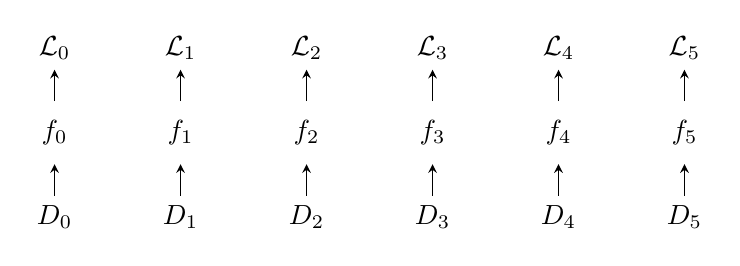
\begin{tikzpicture}
\begin{scope}[scale=0.8]
    
    
    \node (a) at (0,0) [rectangle, rounded corners] {$f_0$};
    \node (b) at (2,0) [rectangle, rounded corners] {$f_1$};
    \node (c) at (4,0) [rectangle, rounded corners] {$f_2$};
    \node (d) at (6,0) [rectangle, rounded corners] {$f_3$};
    \node (e) at (8,0) [rectangle, rounded corners] {$f_4$};
    \node (f) at (10,0) [rectangle, rounded corners] {$f_5$};
    
    \draw[-stealth] (0,0.5) -- (0, 1) node[above] {$\mathcal{L}_0$};
    \draw[-stealth] (2,0.5) -- (2, 1) node[above] {$\mathcal{L}_1$};
    \draw[-stealth] (4,0.5) -- (4, 1) node[above] {$\mathcal{L}_2$};
    \draw[-stealth] (6,0.5) -- (6, 1) node[above] {$\mathcal{L}_3$};
    \draw[-stealth] (8,0.5) -- (8, 1) node[above] {$\mathcal{L}_4$};
    \draw[-stealth] (10,0.5) -- (10, 1) node[above] {$\mathcal{L}_5$};

    
    \draw[-stealth] (0, -1) node[below] {$D_0$} -- (0, -0.5);
    \draw[-stealth] (2, -1) node[below] {$D_1$} -- (2, -0.5);
    \draw[-stealth] (4, -1) node[below] {$D_2$} -- (4, -0.5);
    \draw[-stealth] (6, -1) node[below] {$D_3$} -- (6, -0.5);
    \draw[-stealth] (8, -1) node[below] {$D_4$} -- (8, -0.5);
    \draw[-stealth] (10, -1) node[below] {$D_5$} -- (10, -0.5);
    
\end{scope}
\end{tikzpicture}
\end{center}

	%    \label{fig:progdense_diagram}
	\caption{$n=6$ parameterized functions with losses $\mathcal{L}_i$ and datasets $D_i$.}
\end{figure}{}

Each parameterized function is represented here in its most abstract sense\cite{hinton2015distilling} and need only accept the same input type $x$ and produce the same output dimension to fit within the network. {\color{blue} For instance, unicode encoded string $x = "hello"$ and its semantic representation as a $64x49$ word embedding.} This widened scope ensures participants can be multi-task \cite{kaiser2017model}, use completely distinct computing substrates \cite{alex2014cortical} or train on unique datasets. \cite{lample2019crosslingual}. 

\subsection{Ideal Ranking}

Our goal in this work is to produce a ranking $R = [R_i]$ over these functions where the score $R_i \in R$ represents participant $i$'s information-theoretic significance to the benchmark $\mathcal{B}$. Following Le Cun and others \cite{lecun1989optimalbraindamage,yu2017nisp}, it is reasonable to analytically define this significance by equating it with the cost of removing each component from the network:
\bigskip

\begin{equation}
R_i \approx \ \ \frac{1}{n} \sum_{j}^{n} \sum_{x \in D_j} \Delta F^T(x)_i * H(\mathcal{Q}_j(x)) * \Delta F(x)_i 
\end{equation}

\[ \Delta F (x)_i = [0, ... 0, -f_i(x), 0, ... 0] \]

Where the above is derived using a Taylor series (Appendix 6.1) and $\Delta F (x)_i$ is the {\color{blue} perturbation of the $i^{th}$ node's inputs as a function of it's choice of weights when removing function $f_i$ at the point $x$}. Note, the linear and higher order terms of the Taylor series have been removed following \cite{yu2017nisp} and the remaining term $H(\mathcal{Q}_i)$ is the hessian of our error function. When the error function $\mathcal{Q}$ is the twice-differentiable cross-entropy, then $H(\mathcal{Q}_i)$ is the Fisher information matrix, and $R_i \in R$ is measured as relative entropy: reflects each participants informational significance to the network as a whole.
\bigskip

\subsection{Inter Ranking}
\label{sec:inter-ranking}
It is not possible to compute the ranking score above without access to the parameters of each function in the network. Instead, we use a set of inter-model weights $W = [w_{i_j}]$ where each $w_{i,j}$ is the score attributed to $f_j$ from $f_i$ combined into an $n \times n$ square matrix.
\bigskip

\begin{equation}
w_{ij} = \ \ \sum_{x \in D_i} \Delta F^T(x)_j * H(\mathcal{Q}_i(x)) * \Delta F(x)_j
\end{equation}

\begin{figure}[H]
	\centering
	\hspace*{-2cm}
	\begin{center}

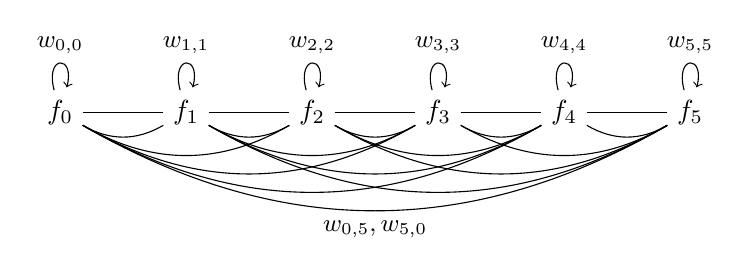
\begin{tikzpicture}


\begin{scope}[scale=0.8]

    \node (a) at (0,0) [rectangle] {$f_0$};
    \node (b) at (2,0) [rectangle] {$f_1$};
    \node (c) at (4,0) [rectangle] {$f_2$};
    \node (d) at (6,0) [rectangle] {$f_3$};
    \node (e) at (8,0) [rectangle] {$f_4$};
    \node (f) at (10,0) [rectangle] {$f_5$};
    
  
    \path[every node/.style={font=\sffamily\small}]
        (a) edge node [right] {} (b)
        (b) edge node [right] {} (c)
        (c) edge node [right] {} (d)
        (c) edge node [right] {} (d)
        (d) edge node [right] {} (e)
        (e) edge node [right] {} (f)


        (a) edge [loop above]  node[above]  {$w_{0,0}$} (a)
        (b) edge [loop above]  node[above]  {$w_{1,1}$} (b)
        (c) edge [loop above]  node[above]  {$w_{2,2}$} (c)
        (d) edge [loop above]  node[above]  {$w_{3,3}$} (d)
        (e) edge [loop above]  node[above]  {$w_{4,4}$}  (e)
        (f) edge [loop above]  node[above]  {$w_{5,5}$}  (f)

        (a) edge [bend right]  (b)
        (a) edge [bend right]  (c)
        (a) edge [bend right]  (d)
        (a) edge [bend right]  (e)
        (a) edge [bend right]  node[below]  {$w_{0,5}, w_{5,0}$}(f)
        (b) edge [bend right]  (c)
        (b) edge [bend right]  (d)
        (b) edge [bend right]  (e)
        (b) edge [bend right]  (f)
        (c) edge [bend right]  (d)
        (c) edge [bend right]  (e)
        (c) edge [bend right]  (f)
        (d) edge [bend right]  (e)
        (d) edge [bend right]  (f)
        (e) edge [bend right]  (f);
    
\end{scope}


\end{tikzpicture}
\end{center}

	%    \label{fig:progdense_diagram}
	\caption{Inter-model contribution weights: $w_{i,j}$ the score attributed to $f_j$ from $f_i$}
\end{figure}{}

%{\color{blue} -- e.g. by using a heuristic to propagate the weights from the final layer of $f_i$ through to the first layer of $f_j$ --}  

The weights can be computed on the fly either approximately \cite{yu2017nisp} or by using the full hessian of the error. We store them on a distributed ledger and allow participants to update them by making changes of bounded size: $W^{t+1}= W^t + \lambda \Delta W$, where $||W_i||_2 < \epsilon$ at block step $t$. We also enforce that the scores in each row sum to 1, $||w||_1 = 1$. {\color{blue} The reasoning for this enforcement is to ensure stake fairness between early movers and newcomers with innovations that enable them to perform better overall.}

The equivalent ranking $R$ (2) can then be computed by normalizing column sum of the weight matrix:
\bigskip

\begin{equation}
R = \frac{1}{n} W^T * \mathbbm{1}
\end{equation}

The problem is that without system-wide access to the model parameters, the computation of $w_{ij}$ (3) is intractable, {\color{blue} as it would require collecting great amounts of information from potentially billions of neurons}. It is reasonable to assume participants will select weights which artificially increase their own rank rather than others in the network. Moreover, since the network remains open, participants may choose to create many spuriously neighbours and rank themselves higher. The remainder of this paper describes our proposal for resolving these issues.
\bigskip

\subsection{Stake}
\label{sec:stake}
The proposed solution begins by introducing a finite resource $ S=[s_i]$, a component's 'stake' in the system, and an inflation mechanism $\tau$ which translates the ranking vector $R$ into additional stake as incentive. 
\bigskip

\begin{equation}
R = \frac{1}{n} W^T \circ S * \mathbbm{1}
\end{equation}

\begin{equation}
S^{t+1} = S^t + \tau * \frac{R}{||R||_2} 
\end{equation}

The $\circ$ here is the Hadamard product between the $n \times n$ matrix $W$ and the $n \times n$ matrix containing $S$ in each column, and $t$ is the time-step referred to in Section~\ref{sec:inter-ranking} (measured in distinct blocks on the distributed ledger). By design (5) increases the importance of those with stake, $s_0 * w_{ij}$. This serves two purposes: 

\begin{enumerate}
	\item New computers can spuriously create new nodes, however this won't game the ranking because the amount of stake they hold is finite.
	\item The resource provides mechanism power.
\end{enumerate}

By providing it to nodes with large rank, this ensures that those with weight must have worked to attain it, or indirectly subsidized those who have done so already. A single staked token would be enough to bootstrap the process. \footnote{The propagation of a resource mocks the flow of the brain-derived neurotrophic factor (BDNF). \cite{Bathina1989neurotrophin}} 
\smallskip

\begin{algorithm}
	\caption{Inflation mechanism}
	\begin{algorithmic} 
		
		\REQUIRE $S = \ [n \times 1] \ \textrm{Stake Vector}$
		\REQUIRE $W = \ [n \times n] \ \textrm{Weight Matrix}$
		\REQUIRE $\tau > 0 \ \textrm{inflation rate}$
		\WHILE{$\text{TRUE}$}
		\STATE $W = W + \lambda \Delta W$
		\STATE $R = \frac{1}{n} W^T \circ S * \mathbbm{1}$
		\STATE $S = S + \tau * \frac{R}{||R||_2}  $
		\ENDWHILE
	\end{algorithmic}
\end{algorithm}
\smallskip

\subsection{Competitive weights}
\label{sec:competitive_weights}
While stake provides some protection against malicious actors, it does not ensure weights are set accurately. Our solution begins by introducing competition for connectivity within the network. Nodes that underweight are punished by having inputs from the network masked to zero~(\ref{eq:7}), {\color{blue} which in turn would punish the loss function}. To frame this market we borrow the continuous differential activation function $\sigma$ with range $(0,1)$. Under a choice of weights $W_i$ the inputs to component $i$ are:
\bigskip

\begin{equation}
\label{eq:7}
F_W(x) =  [f_0(x) * \sigma(s_i * w_{i,0} - \mu_0),  ... , f_n(x) * \sigma(s_i * w_{i,n} - \mu_n)]
\end{equation}

\begin{equation}
\sigma =  \frac{1}{ 1 + e^{-\frac{x}{T}} }
\end{equation}

Here, the shift term $\mu_j$ is the average of the weights in each column $\mu_j = (\frac{1}{n}) \sum_{i}^{n}{s_i * w_{i,j}}$, and the activation function is the temperature scaled sigmoid. Because the allocation mechanism is standard across the network it is possible for each participants to compute both $\frac{\partial \mathcal{L}_i}{\partial W_i}$ and $\frac{\partial R_i}{\partial W_i}$. Computers may augment their usual training framework, for instance, Tensorflow, with the allocation mechanism shown here. 
\bigskip

\subsection{Running the network}

The steps to run a network participant are:
\begin{enumerate}
	
	\item Participant defines its dataset $D_i$, loss $\mathcal{L}_i$ and parameterized function $f_i$
	\item  At each training iteration the participant broadcasts batches of examples from $D_i$ to its peers $[\textit{batch\_size}, x]$
	\item Responses $F(x)$ from the network produce a loss-gradient $\frac{\partial \mathcal{L}}{\partial F}$ which back-propagates through $f_i$ and out to the network.
	\item  During 2 and 3 the participant competitively selects the weights for their row $w_{ij} \in W$.
	\item  Participants submit changes to the weights $\Delta W_i$ which, in-turn changes the ranking and induces inflation $\tau * R$.
	\item  {\color{blue} After steps 1-5 have been performed multiple times}, participants disconnect and verify the model in a normal manner.
\end{enumerate}

Peers only communicate with computers that hold stake as a consequence of section~\ref{sec:competitive_weights}. Those that fail to produce value will be pruned naturally as participants learn to differentiate signal from noise.

\subsection{Conditional computation}

As the network grows, outward bandwidth will become the major bottleneck. Components learn to trim outward bandwidth by employing a Sparsely-Gated Mixture-of-Experts (SGMoE) \cite{shazeer2017outrageously} layer at the input. The gating layer determines a sparse combination of children to query for each example and then re-joins them using the the gating weights $g_j(x)$. The combined gated inputs are fed as input to the local function: 

\begin{equation}
f_i = f_i(G(x)) \ \ \ \  \textrm{ }
\end{equation}

\begin{equation}
G(x) = [ ..., g_j(x) * f_j(x), ...]
\end{equation}


The layer cuts outward bandwidth, querying only a small subset of peers for each example. The gating function is trainable w.r.t to the loss and its weights act as a proxy for importance $w_{ij} \in W$. This method has been shown to drastically increase the potential for outward bandwidth in datacenter training,\cite{shazeer2017outrageously} and has been investigated in a peer-to-peer (P2P) setting as well \cite{Riabinin2020learningathome}


\subsection{Extracting knowledge}

Inter-node dependence in the network is broken using distillation\cite{hinton2015distilling}, a compression and knowledge technique in which a smaller model -- the student - mimics the behaviour of an ensemble. We employ this technique over the gating ensemble (10) where the student model learns to minimize the cross-entropy (shown below as KL) between the logits produced by the gating network and its predicted distribution. \cite{Sanh2019DistilBERT}
\smallskip

\begin{equation}
\textrm{distillation loss} = \text{KL}_D(\text{dist}(x), G(x)) 
\end{equation}

We use the distilled model as proxy to cut recursive calling between each components rather than query farther into the network. If models go offline, their peers can use their distilled versions in-place. Private data can be validated over the distilled models instead of querying the network. Eventually, components can fully disconnect from the network using the distilled inputs to validate and inference the models offline.
\smallskip

\begin{figure}[H]
	\centering
	\hspace*{0cm}
	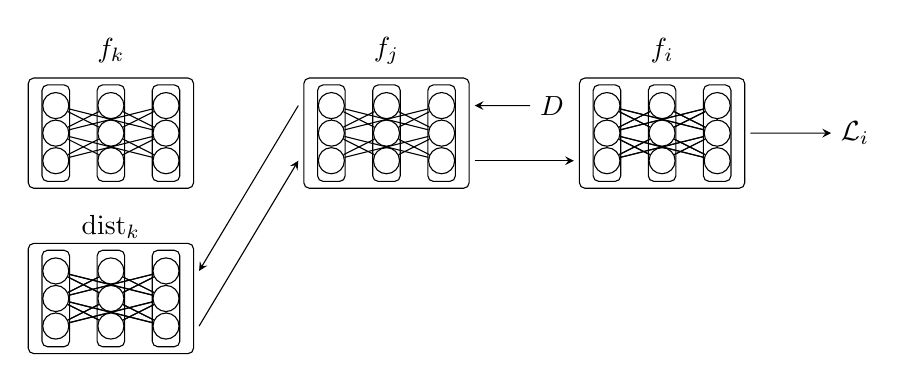
\begin{tikzpicture}


\begin{scope}[scale=0.7]

    \node[] at (1,2) {$f_j$};
    \node[] at (-4,2) {$f_k$};
    \node[] at (6,2) {$f_i$};
    
    \node[] at (-4,-1.2) {$\text{dist}_k$};

    

    %\draw[-stealth] (-7,3) node[below] {$\mathbf{M_1}$} -- (-5.5, 0.5);
    %\draw[-stealth] (-2.5, 0.5) -- (-1.5, 1.75) node[above] {$\mathcal{L}_k$};
    %\draw[-stealth] (2.5, 0.5) -- (3.5, 1.75) node[above] {$\mathcal{L}_j$};
    
    \node[] (m) at (4, 1) {$D$};
    \node[] (l) at (9.5, 0.5) {$\mathcal{L}_i$};
    
    \draw[-stealth] (m) -- (2.6, 1);
    \draw[-stealth] (7.6, 0.5) -- (l);

    
   % \draw[-stealth] (7.5, 0.5) -- (8.5, 1.75) node[above] {$\mathcal{L}_i$};
    
    \draw[-stealth] (2.6, 0) -- (4.4, 0);
    \draw[-stealth] (-0.6, 1) -- (-2.4, -2.0);
    \draw[-stealth] (-2.4, -3) -- (-0.6, 0);
    

    \foreach \x in {0,...,2}
        {
        \foreach \y in {0,...,2} 
            {
            \node[circle, draw, scale=1] (\x\y) at (\x, \y * 0.5) {};
            }
        \draw[rounded corners=2] (\x - 0.25, 1.375) rectangle ++(0.5, -1.75);
        }
    \draw[rounded corners=2] (-0.5, -0.5) rectangle ++(3, 2);
    
    
    \foreach \x in {0,...,2}
        {
        \foreach \y in {1,2}
            {
            \pgfmathsetmacro\yi{int(\y - 1)}
            \draw (\x\yi)edge(0\y);
            \draw (\x\yi)edge(1\y);
            \draw (\x\yi)edge(2\y);
            }
        }
        
     \foreach \x in {0,...,2}
        {
        \foreach \y in {0,...,2} 
            {
            \node[circle, draw, scale=1] (\x\y) at (\x - 5, \y * 0.5) {};
            }
        \draw[rounded corners=2] (\x - 0.25 - 5, 1.375) rectangle ++(0.5, -1.75);
        }
    \draw[rounded corners=2] (-0.5 - 5, -0.5) rectangle ++(3, 2);

    
    \foreach \x in {0,...,2}
        {
        \foreach \y in {1,2}
            {
            \pgfmathsetmacro\yi{int(\y - 1)}
            \draw (\x\yi)edge(0\y);
            \draw (\x\yi)edge(1\y);
            \draw (\x\yi)edge(2\y);
            }
        }
        
    \foreach \x in {0,...,2}
        {
        \foreach \y in {0,...,2} 
            {
            \node[circle, draw, scale=1] (\x\y) at (\x + 5, \y * 0.5) {};
            }
        \draw[rounded corners=2] (\x - 0.25 + 5, 1.375) rectangle ++(0.5, -1.75);
        }
    \draw[rounded corners=2] (-0.5 + 5, -0.5) rectangle ++(3, 2);

    
    \foreach \x in {0,...,2}
        {
        \foreach \y in {1,2}
            {
            \pgfmathsetmacro\yi{int(\y - 1)}
            \draw (\x\yi)edge(0\y);
            \draw (\x\yi)edge(1\y);
            \draw (\x\yi)edge(2\y);
            }
        }
        
        
    %  \foreach \x in {0,...,2}
    %     {
    %     \foreach \y in {0,...,2} 
    %         {
    %         \node[circle, draw, scale=1] (\x\y) at (\x, \y * 0.5 - 4) {};
    %         }
    %     \draw[rounded corners=2] (\x - 0.25, 1.375 - 4) rectangle ++(0.5, -1.75);
    %     }
    % \draw[rounded corners=2] (-0.5, -0.5 - 4) rectangle ++(3, 2);

    
    \foreach \x in {0,...,2}
        {
        \foreach \y in {1,2}
            {
            \pgfmathsetmacro\yi{int(\y - 1)}
            \draw (\x\yi)edge(0\y);
            \draw (\x\yi)edge(1\y);
            \draw (\x\yi)edge(2\y);
            }
        }
        
     \foreach \x in {0,...,2}
        {
        \foreach \y in {0,...,2} 
            {
            \node[circle, draw, scale=1] (\x\y) at (\x - 5, \y * 0.5 - 3) {};
            }
        \draw[rounded corners=2] (\x - 0.25 - 5, 1.375 - 3) rectangle ++(0.5, -1.75);
        }
    \draw[rounded corners=2] (-0.5 - 5, -0.5- 3) rectangle ++(3, 2);

    
    \foreach \x in {0,...,2}
        {
        \foreach \y in {1,2}
            {
            \pgfmathsetmacro\yi{int(\y - 1)}
            \draw (\x\yi)edge(0\y);
            \draw (\x\yi)edge(1\y);
            \draw (\x\yi)edge(2\y);
            }
        }
        
    %  \foreach \x in {0,...,2}
    %     {
    %     \foreach \y in {0,...,2} 
    %         {
    %         \node[circle, draw, scale=1] (\x\y) at (\x + 5, \y * 0.5 - 4) {};
    %         }
    %     \draw[rounded corners=2] (\x - 0.25 + 5, 1.375 - 4) rectangle ++(0.5, -1.75);
    %     }
    % \draw[rounded corners=2] (-0.5 + 5, -0.5- 4) rectangle ++(3, 2);

    
    \foreach \x in {0,...,2}
        {
        \foreach \y in {1,2}
            {
            \pgfmathsetmacro\yi{int(\y - 1)}
            \draw (\x\yi)edge(0\y);
            \draw (\x\yi)edge(1\y);
            \draw (\x\yi)edge(2\y);
            }
        }
        
 
    
    
    % \foreach \y in {0,...,2}
    %     {
    %     \foreach \x in {0,...,2} 
    %         {
    %         \pgfmathsetmacro\xi{(6 + \x*0.5)}
    %         \node[circle, draw] (\x\y) at (\xi,\y) {};
    %         }
    %     \draw[rounded corners=2] (6 + -0.375,\y+0.25) rectangle ++(1.75,-0.5);
    %     }
    % \draw[rounded corners=2] (6 + -0.5, -0.4) rectangle ++(2, 2.8);

    
    % \foreach \x in {0,...,2}
    %     {
    %     \foreach \y in {1,2}
    %         {
    %         \pgfmathsetmacro\yi{int(\y - 1)}
    %         \draw (\x\yi)edge(0\y);
    %         \draw (\x\yi)edge(1\y);
    %         \draw (\x\yi)edge(2\y);
    %         }
    %     }
        
    % \draw[-stealth] (6 + 0.5,-1) node[below] {$\mathbf{M_1}$} -- (6 + 0.5,-0.5);
    % \draw[-stealth] (6 + 0.5,2.5) -- (6 + 0.5,3) node[above] {$\mathcal{L}_1$};
    
    
    % \foreach \y in {0,...,2}
    %     {
    %     \foreach \x in {0,...,2} 
    %         {
    %         \pgfmathsetmacro\xi{(6 + \x*0.5)}
    %         \node[circle, draw] (\x\y) at (\xi,-6 +  \y) {};
    %         }
    %     \draw[rounded corners=2] (6 + -0.375, -6 + \y+0.25) rectangle ++(1.75,-0.5);
    %     }
    % \draw[rounded corners=2] (6 + -0.5, -6 + -0.4) rectangle ++(2, 2.8);

    
    % \foreach \x in {0,...,2}
    %     {
    %     \foreach \y in {1,2}
    %         {
    %         \pgfmathsetmacro\yi{int(\y - 1)}
    %         \draw (\x\yi)edge(0\y);
    %         \draw (\x\yi)edge(1\y);
    %         \draw (\x\yi)edge(2\y);
    %         }
    %     }
        
    % \draw[-stealth] (6 + 0.5, -6 + -1) node[below] {$\mathbf{M_2}$} -- (6 + 0.5, -6 +  -0.5);
    % \draw[-stealth] (6 + 0.5, -6 + 2.5) -- (6 + 0.5, -6 + 3) node[above] {$\mathcal{L}_2$};
    
    
    %  \foreach \y in {0,...,2}
    %     {
    %     \foreach \x in {0,...,2} 
    %         {
    %         \pgfmathsetmacro\xi{(12 + \x*0.5)}
    %         \node[circle, draw] (\x\y) at (\xi, -6 +  \y) {};
    %         }
    %     \draw[rounded corners=2] (12 + -0.375, -6 + \y+0.25) rectangle ++(1.75,-0.5);
    %     }
    % \draw[rounded corners=2] (12 + -0.5, -6 + -0.4) rectangle ++(2, 2.8);

    
    % \foreach \x in {0,...,2}
    %     {
    %     \foreach \y in {1,2}
    %         {
    %         \pgfmathsetmacro\yi{int(\y - 1)}
    %         \draw (\x\yi)edge(0\y);
    %         \draw (\x\yi)edge(1\y);
    %         \draw (\x\yi)edge(2\y);
    %         }
    %     }
        
    % \draw[-stealth] (12 + 0.5, -6 + -1) node[below] {$\mathbf{M_3}$} -- (12 + 0.5, -6 +  -0.5);
    % \draw[-stealth] (12 + 0.5, -6 + 2.5) -- (12 + 0.5, -6 + 3) node[above] {$\mathcal{L}_3$};
    
    
    % \draw[-stealth] (5, 1) -- (2, 1);
    % \draw[-stealth] (5, -5) -- (2, -1);
    % \draw[-stealth] (11, -5) -- (8, -1);
    % \draw[-stealth] (11, -5) -- (8, -5);
    
    % \node[] at (-1,2) {$f_0$};
    % \node[] at (5,2) {$f_1$};
    % \node[] at (5,-4) {$f_2$};
    % \node[] at (11,-4) {$f_3$};

    
\end{scope}


\end{tikzpicture}
	%    \label{fig:progdense_diagram}
	\caption{Queries propagate to depth=1 before the distilled model is used.}
\end{figure}{}

\section{Analysis}
\label{analysis}

We consider the scenario where participants are not honestly reporting the significance of their peers. The network is progressing at discrete timesteps $t$ and it is reasonable to assume that each participant is attempting to maximize their subjective payoff over these steps.

\subsection{Payoff Model}

The staking system in Section~\ref{sec:stake} gives participants incentive to maximize their self-weight $w_{ii}$ while the competitive connectivity described in Section~\ref{sec:competitive_weights} makes it costly for participants to decrease the remaining weights $w_{ij}$ in their row. Since the row must sum to 1, we have a trade-off in two terms:

\begin{enumerate}
	\item A utility term attached to the loss $U(\mathcal{L}(W))$.
	\item The token emission via inflation $\tau * R_i(W)$. 
\end{enumerate}

Both of these are functions of the weights and, without loss of generality, measured in similar units:
\bigskip

\begin{equation}
P_i (W) = U_i(\mathcal{L}_i(W)) + \tau * R(W)_i
\end{equation}
\smallskip

It is reasonable to assume payoff maximizing participants will use $P_i$ as their objective during training. This can be computed using standard tools since both terms $U(\mathcal{L}_i(W))$ and $R(W)_i$ are fully continuous and differentiable. The system can be characterized as a competitive gradient descent game where participants are making steps $\Delta W_i = \frac{\partial P_i}{\partial W_i}$. In appendix 6.2 we prove that this strategy is regret-free and achieves the best expected payoff in hindsight. This assumption is also generally employed in smooth markets \cite{balduzzi2020smooth}. The iterative descent thus follows:
\smallskip


\begin{equation}
W^{t+1} = W^{t} + \lambda \Delta W 
\end{equation}
\smallskip


\begin{equation}
\Delta W = [\frac{\partial P_0}{\partial W_0} ; ... ;\frac{\partial P_n}{\partial W_n}]
\end{equation}
\smallskip

\subsection{Empirical Model}

Without access to the running network we evaluate our system using an empirical model. To derive the gradient steps in this model $\frac{\partial P_i}{\partial W_i}$ we make the following assumptions: 

\begin{enumerate}
	\item The utility functions are continuous-differentiable and are bounded by their first order derivatives $\frac{\partial U}{\partial \mathcal{L}} = \alpha$.
	\item  The network is converged to a local minimum in the inputs $\frac{\partial\mathcal{L}}{\partial F} = 0$.
\end{enumerate}  

The first assumption is approximate for small changes of continuous functions and the second assumption is realistic after extended training. In Appendix 6.2 we derive the following gradient step:
\smallskip

\begin{equation}
\frac{\partial P}{\partial W} = \frac{\alpha}{\tau} * \frac{\partial L}{\partial W} + \frac{\partial R}{\partial W}
\end{equation}
\smallskip


\begin{equation}
\frac{\partial L}{\partial W} = \frac{\partial}{\partial W} [(F_W - F_{W_0})^T * H( \mathcal{L}(F)) * (F_W - F_{W_0})] 
\end{equation}
\smallskip

Here $F_W$ is the masked inputs from Section~\ref{sec:competitive_weights}. $(F_W - F_{W_0})$ is the difference in the mask between the choice of weights $W$ and the weights at the minimum $W_0$ and $H( \mathcal{L}(F))$ is the $[n \times n]$ hessian of the loss over inputs $F$. This formulation is both intuitive and useful: the gradient term $\frac{\partial L}{\partial W}$ measures the change in loss for any choice of weights. Additionally, it also allows us to compute the ranking for simulated hessian terms.
\smallskip

The remainder of the network is deterministic, and can be described by a choice of $\theta = [\alpha, \tau, \lambda, n, \sigma, T, S, W, H]$. For instance, the secondary term, $\frac{\partial R}{\partial W}$ can be computed-directly from Section~\ref{sec:stake} and only depends on the stake vector $S$ and weights $W$.
\smallskip

\section{Experiments}
\label{experiments}
\begin{figure}[!htb]
	\centering
	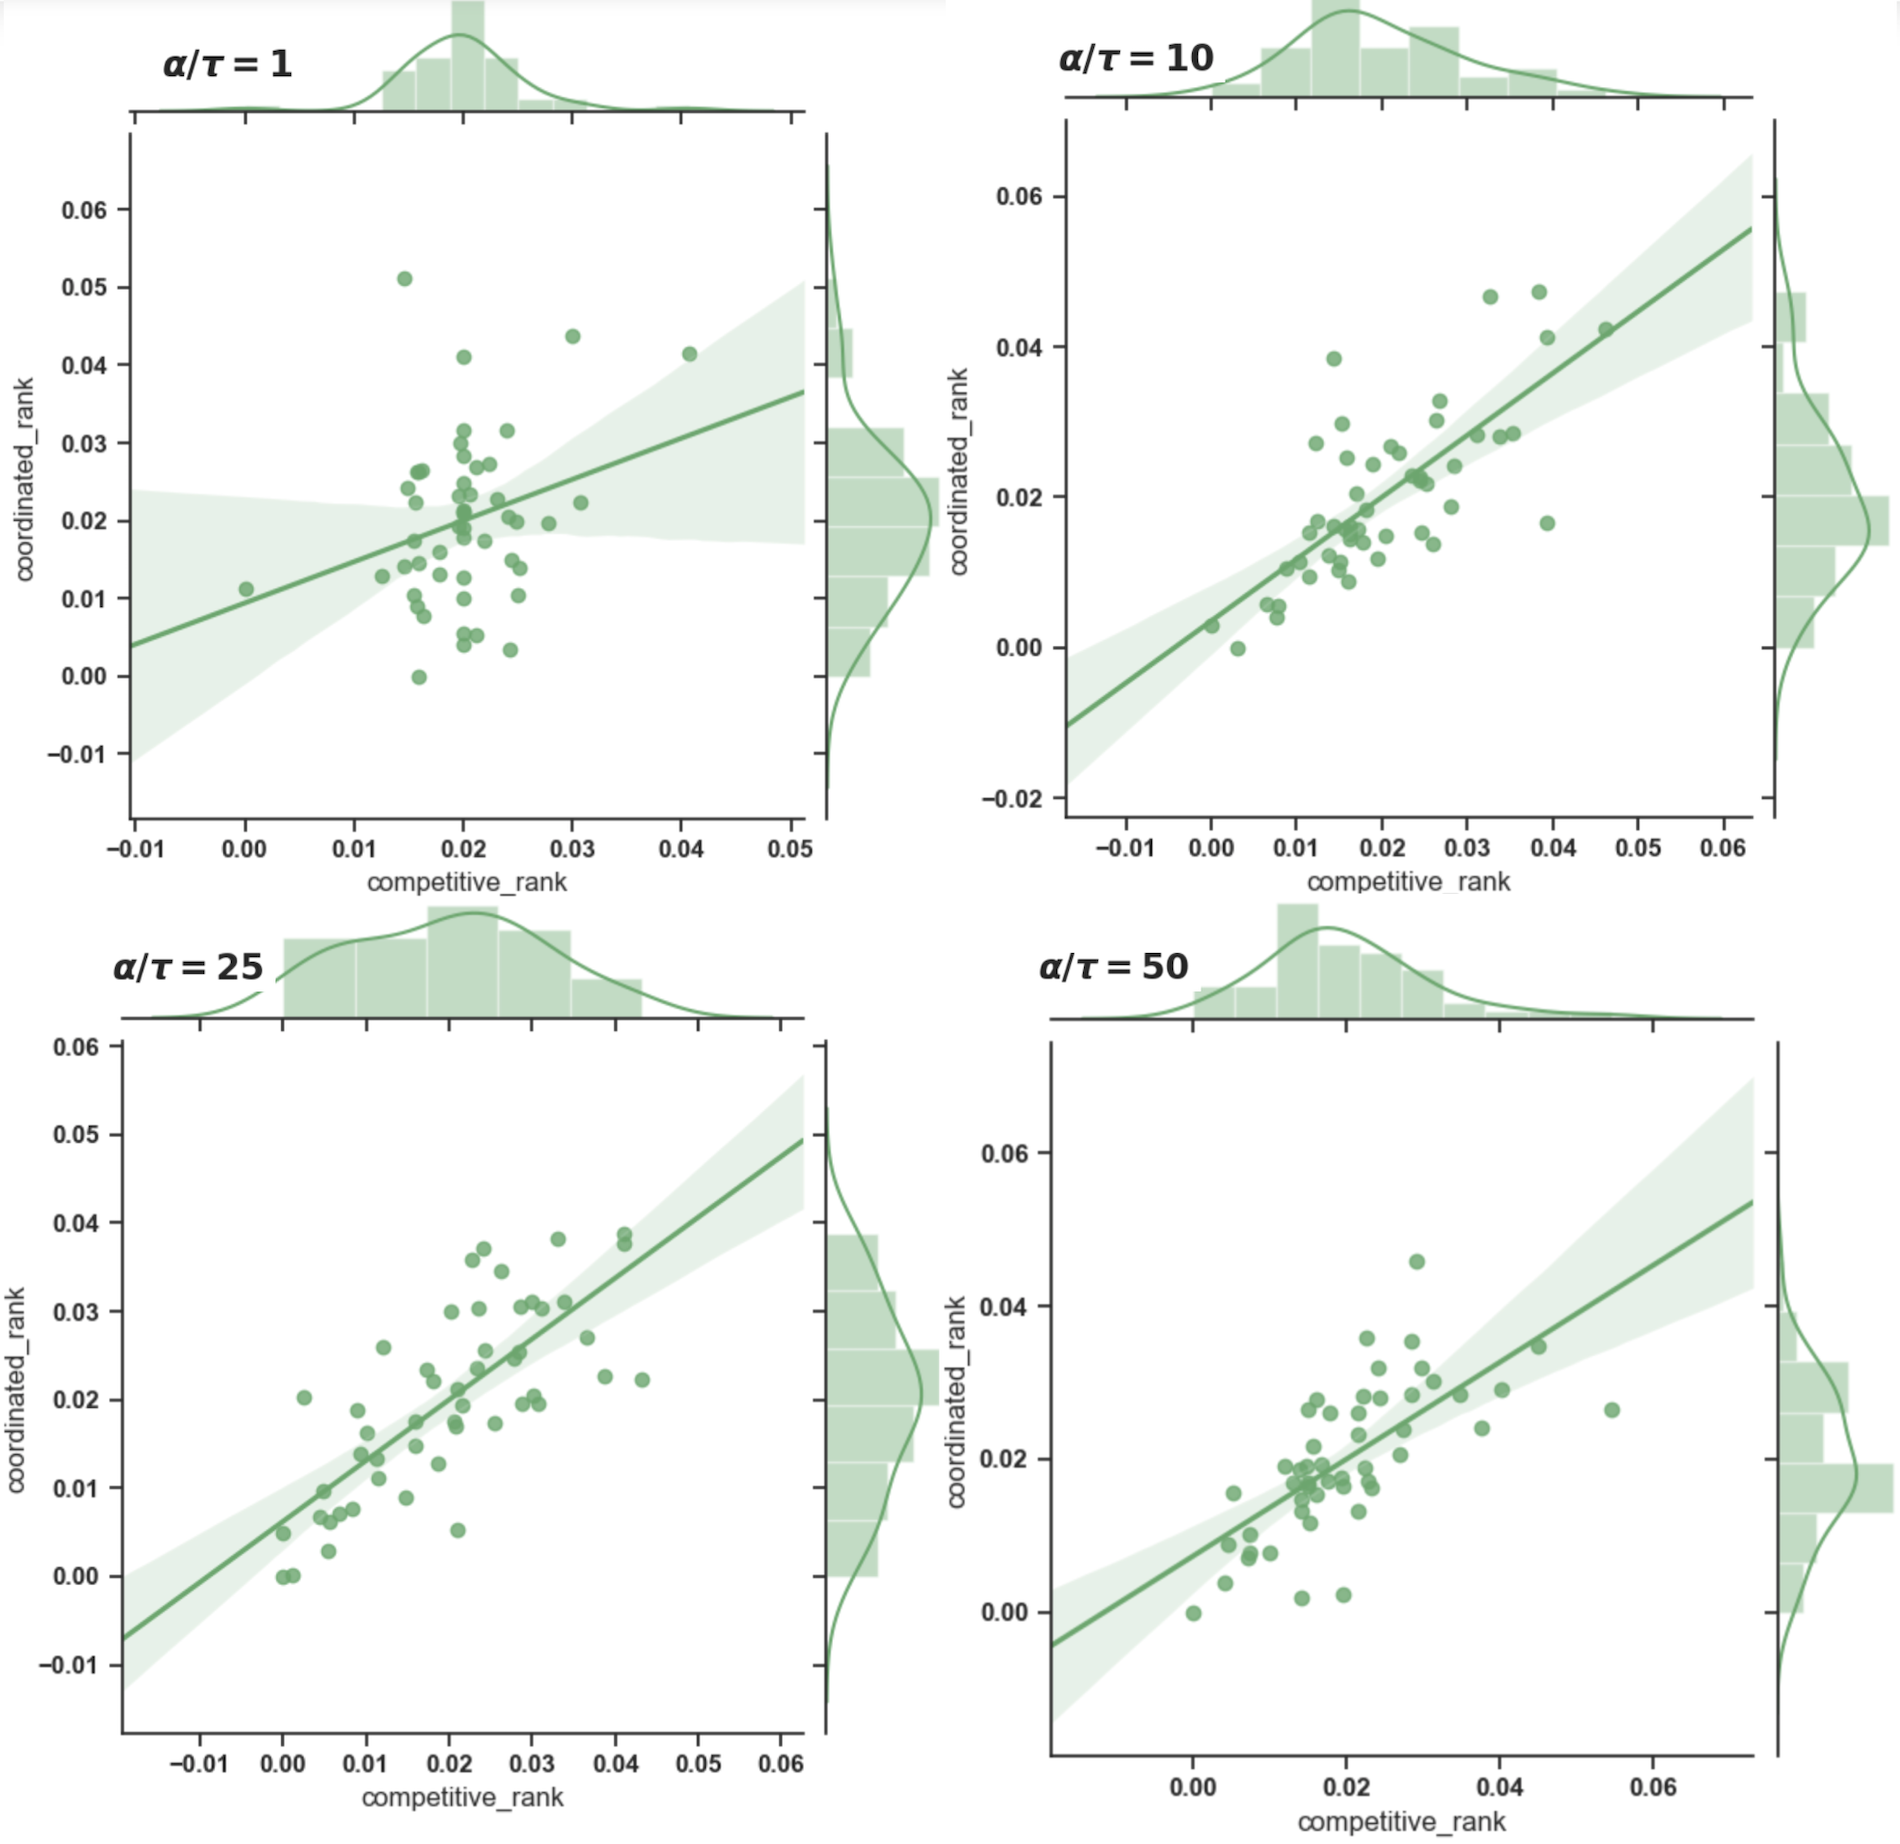
\includegraphics[scale=.34]{images/c_vs_c_nice.png}
	\caption{Correlations between the competitive rank and coordinated rank for $\frac{\alpha}{\tau} \in \{1, 10, 25, 50\}$. For low values of $\frac{\alpha}{\tau}$ the weights converge to the identity: the state where peers are fully disconnected. }
	\label{coordvscomp}
\end{figure}
\smallskip

\begin{figure}[!htb]
	\centering
	\includegraphics[scale=.27]{images/adaptive_tau.png}
	\caption{(i) Left: the ratio between the main diagonal and the remainder of the weights. Right: the adaptive $\tau$ parameter converging onto the target. The weight matrix sparsity is a proxy for the ranking accuracy which we see in Figure~\ref{coordvscomp}. As sparsity converges onto the target the ranking is also improving.}
	\label{adaptive_tau}
\end{figure}


To generate sample statistics from the network, we first select $[\alpha, \tau, \lambda, S, \sigma, T, n] \in \theta$, then we generate random positive semi-definite hessians $H$, and random uniform initial weights $W_0$. For each parameterization we discover the competitive ranking by converging the system to a Nash-equilibrium: an equilibrium where no individual can vary from their set of weights and stand to gain. \cite{dtting2017optimal} To find this equilibrium, we use the competitive descent strategy described in (14) and compute the gradient terms from (15). In each trial we use a learning rate $\lambda = 0.005$ and stop when the gradient terms are bounded by $\epsilon$ or the steps exceed $1000 \times n$. The competitive ranking $R^*$ at this point follows from (4) and can be compared to the idealized score in $R$ from (2).
\smallskip

We are interested in the correlation between $R^*$ and $R$ as we vary the ratio $\alpha$ and $\tau$, this ratio is explicit in (15) where the fraction relates the two gradient terms. Intuitively the ratio is between the value of minimizing the loss and maximizing revenue from inflation. Since this effects the ranking, we show this trade-off for various choices in Figure~\ref{coordvscomp}. 
\smallskip

Finally, in Figure-\ref{adaptive_tau} we implement an adaptive-$\tau$ strategy where the network varies the inflation rate. Initial inflation is zero and then increases until the weights begins to converge towards the main diagonal $w_{ii}=1$. We measure the sparsity $sparsity = sum(W_{dg})/sum(W)$, the ratio between the main diagonal and the remaining weights. As sparsity increases we push the market equilibrium by decreasing $\tau$. Figure shows this adaptive convergence for $\alpha=1$ with a sparsity target of 1.
\smallskip

\subsection{Discussion}

Figure~\ref{coordvscomp} shows the relationship between the idealized rank and the competitive rank as a function of $\frac{\alpha}{\tau}$. Figure-\ref{coordvscomp}-a, $\frac{\alpha}{\tau} = 1$ shows the case where this ratio negatively effects the ranking accuracy. Here, all components have set $w_{ii} = 1$ and the resulting scores for all participants has converged to $1/n$. When this occurs, the system could decrease the inflation rate $\tau$ and push the network towards the high information markets seen in Figure-\ref{coordvscomp}-b, c, and d. Figure-\ref{adaptive_tau} shows a basic implementation of this where $\tau$ adapts to the ratio between the row-sums and the main-diagonal. By lowering inflation, it subsequently 'costs less' to connect with peers. Profit maximizing nodes automatically adjust to the change and the system converges back towards an accurate ranking. Those with high ranks will oppose inflation decreased, while those with low ranks will welcome it. The equilibrium found in this meta game will most certainly depend on the number of participants, key to both the ranking accuracy and the market at its core. However, we leave this analysis for a follow up paper. 
\smallskip

\section{Conclusion}
\label{conclusion}
We have proposed an inter-model benchmark that can run in a P2P setting outside of a trusted environment. We started with a typical machine learning framework defined by a set of functions with their losses over given datasets, then derived an idealized ranking score. The measure produced an information theoretic score that new participants can improve by learning how to be useful to their peers. However, the system is incomplete without a mechanism that prevents participants from ranking dishonestly. To resolve this, we proposed an incentive scheme and a differential allocation system over the network weights. The system allows the participants to train for connectivity in the graph. Following this, we described how to increase the outward bandwidth in the system using a trainable gating network and how to cut dependence between nodes using distillation. Finally we showed how increasing the number of nodes in the system and fixing the inflation mechanism properly ensured that the resulting rank scores would correlate with those found in a idealized setting. While this is true, stake in the system holds value as a means to drive what the network learns. That benchmark is continually being solved by the participants, compounding what has been learned before and making it available to new learners in the system.

%\begin{itemize}
%	\item $n$: The number of nodes e.g. n=100. 
%	\item $\alpha$: The first order utility derivative $\frac{\partial U}{\partial \mathcal{L}} = \alpha$.
%	\item $\tau$: The block-inflation rate: $S^{t+1} = S^t + \tau * R$.
%	\item $\lambda$: The weight matrix learning rate: $W^{t+1} = W^t + \lambda \Delta W$.
%	\item $\sigma$, $T$: The activation function and temperature: $\sigma =  \frac{1}{ 1 + e^{-\frac{x}{T}} }$
%	\item $S$: The stake vector $[1 \times n]$
%	\item $W_0$: A initial weight matrix $ [n \times n]$
%	\item $H( \mathcal{L}(F))_i$: For each $f_i$, the hessian of the loss $L_i$ over inputs $F(x)$ $ n \times [n \times n]$
%\end{itemize}

\section{Broader Impact}
In order to provide a balanced perspective, authors are required to include a statement of the potential broader impact of their work, including its ethical aspects and future societal consequences. Authors should take care to discuss both positive and negative outcomes.

\small
\bibliographystyle{IEEEtran}
\bibliography{references}        % References

\section{Appendix}

\subsection{Deriving the idealized ranking.}

We approximate the change in the benchmark $\Delta \mathcal{B}$ at a local minimum under a perturbation $\Delta F (x)_i = [ ..., -f_i(x) , ...]$ reflecting the removal of the $i^{th}$ node.
\smallskip

\begin{equation}
\Delta \mathcal{B} = \mathcal{B}(F + \Delta F_i) - \mathcal{B}(F) = \sum_{i}^{n} \mathcal{L}_i(F + \Delta F_i) - \mathcal{L}_i(F)
\end{equation}

\begin{equation}
\mathcal{L}_i(F + \Delta F_i) - \mathcal{L}_i(F) \approx \frac{\partial \mathcal{L}_i}{\partial F} * \Delta F_i + \frac{1}{2} \Delta F_i^T * H(\mathcal{L}_i) * \Delta F_i + O(\Delta F_i^3)
\end{equation}

(17) follows from the definition of the benchmark $\mathcal{B}$ and (18) follows from a Taylor series under the perturbation $\Delta F (x)_i$. Note that the first term $\frac{\partial \mathcal{L}_i}{\partial F}$ is zero at the local minimum and the higher order term $O(\Delta F_i^3)$ can be ignored for sufficiently small perturbations. These assumptions are also made by \cite{lecun1989optimalbraindamage} and \cite{yu2017nisp}. Note that $\mathcal{L}_i$ is an expectation over the dataset $D_i$, and all terms are evaluated at a point $x$ so we have:
\smallskip

\begin{equation}
\Delta \mathcal{B} \approx \sum_{i}^{n} \sum_{x \in D_i}  \Delta F_i^T(x) * H(\mathcal{Q}_i(x)) * \Delta F_i(x) 
\end{equation}

Here the hessian over the error function $H(\mathcal{Q}_i(x))$ and the summation over the dataset $\sum_{x \in D_i}$ have been appropriately substituted. The constant factor $\frac{1}{2}$ can be removed and this leaves our result.
\smallskip

\subsection{Deriving the weight convergence game.}

\subsection{Theorem}

For choice of Hessians $H(\mathcal{L}(F))$ the network convergence-game can be described with the following linear relationship between gradient terms:

\begin{equation}
\frac{\partial P}{\partial W} = \frac{\alpha}{\tau} * \frac{\partial L}{\partial W} + \frac{\partial R}{\partial W}
\end{equation}
\smallskip

With the gradient of the loss:

\begin{equation}
\frac{\partial L}{\partial W} = \frac{\partial}{\partial W} [(F_W - F_{W_0})^T * H( \mathcal{L}(F)) * (F_W - F_{W_0})] 
\end{equation}
\smallskip


\subsection{Setup}

We analyze the system by characterizing the behaviour of participants via their payoff in two terms:

\begin{enumerate}
	\item The utility attached to that participant’s loss as a function of their weights $U(L(W))$. $U$ is assumed roughly linear for small change in the weight matrix, $U(\mathcal{L}) = \alpha*\mathcal{L}$, and $\frac{\partial U}{\partial \mathcal{L}} = \alpha$.
	\item The network is converged to a local minimum in the inputs $\frac{\partial\mathcal{L}}{\partial F} = 0$.
\end{enumerate} (1)  and (2)  From the payoff formulation in 6.3 we write:
\smallskip

\begin{equation}
P(W) = \alpha * L(W) + \tau * R(W)
\end{equation}
\smallskip

Note, the utility function and emission were measured in similar units and so $\alpha$ is the \textit{price} of each unit change in loss. The analysis just supposes such a score exists, not that it can be computed. Participants are selecting their weights by making gradient steps $\Delta W_i = \frac{\partial P_i}{\partial W_i} = \frac{\partial U_i}{\partial W_i} + \tau * \frac{\partial R_i}{\partial W_i}$ as to maximize their local payoff. For brevity we omit the subscript $i$ for the remainder of the analysis. Consider a Taylor expansion of the loss under a change $\Delta F$ in the inputs.

\begin{equation}
\mathcal{L}(F + \Delta F) = L(F) + \frac{\partial \mathcal{L}}{\partial F} \Delta F + \frac{1}{2} \Delta F * H( \mathcal{L} (F) ) * \Delta F + O(\Delta F^3) 
\end{equation}

The first linear term $\frac{\partial L}{\partial F}$ is zero and the higher order terms are removed for sufficiently small perturbations in $F$. We then perform a change of variable $F = F_{W_0}$, and $\Delta F = F_{W_1} - F_{W_0}$ where is $W_0$ are the current set of weights and $W_1$ are another choice such that $F_{W_0}$ and $F_{W_1}$ are those inputs masked by $W_0$ and $W_1$ according to (7). Substituting this into (23):

\begin{equation}
\mathcal{L}(F_{W_1}) = L(F_{W_0})) + \frac{1}{2} (F_{W_1} - F_{W_0})^T * H( \mathcal{L}(F)) * (F_{W_1} - F_{W_0}) 
\end{equation}

The function $\mathcal{L}(F_{W_1})$ is simply an approximation of the loss for any choice of weights $W_1$ given that the network has converged under $W_0$. Finally, by the $\alpha$-linear assumption of the utility we can attain the following: 

\begin{equation}
\frac{\partial U}{\partial W} = \alpha * \frac{\partial L}{\partial W} = \alpha \frac{\partial}{\partial W} [(F_W - F_{W_0})^T * H( \mathcal{L}(F)) * (F_W - F_{W_0}) ]
\end{equation}

Note that we've dropped the subscript $W_1$,  $L(F_{W_0}))$ is constant not depending on the choice of weights, and the fraction $\frac{1}{2}$ has been removed. The remaining term $\frac{\partial R}{\partial W}$ is derivable via the ranking ranking function in Section~\ref{sec:inter-ranking}.  Finally, dividing both terms by $\tau$ shows the result:

\begin{equation}
\frac{\partial P}{\partial W} \approx \frac{\alpha}{\tau} * \frac{\partial L}{\partial W} + \frac{\partial R}{\partial W}
\end{equation}

\begin{equation}
\frac{\partial L}{\partial W} = \frac{\partial}{\partial W} [(F_W - F_{W_0})^T * H( \mathcal{L}(F)) * (F_W - F_{W_0})] 
\end{equation}
\smallskip


\subsection{Deriving the ex-post zero-regret step.}

Consider the system described above. A set of $n$ nodes are changing the weights in the ranking matrix $W$ iteratively using gradient descent with learning rate $\lambda$. $W^{t+1} = W^t + \lambda \Delta W$. Here, the change of weights is $\Delta W = [\Delta w_0, ... , \Delta w_n]$ where each $\Delta w_i$ is the weight change pushed by node $i$. Each node is attempting to competitively maximize it's payoff as a function of the weights $P_i(W)$.
\smallskip


\subsubsection{Definition}

The ex-post regret for a single step is the maximum difference in loss between the chosen step $\Delta w_i$ and all alternative $\Delta w_i^*$. The \textit{expected} ex-post regret is this difference in expectation, where the expectation is taken over all choices $\Delta w_j$'s chosen by other participants \cite{dtting2017optimal}.
\smallskip


\begin{equation}
\textrm{rgt}_i = E_{\Delta w_j} [ \max_{\Delta w_i^*} [P_i(\Delta w_i^*) - P_i(\Delta w_i)] ] 
\end{equation}

\subsubsection{Theorem}

For sufficiently small $\lambda$, the expected ex-post regret for strategy $\Delta w_i = \frac{\partial P}{\partial w_i}$ is 0.
\smallskip

\subsubsection{Proof}

Consider Taylor's theorem at the point $W$ for the payoff function $P$ under a change in weights $W^* = W + \lambda \Delta W$. There exists a function $h(W^*)$ such that in the limit as, $W^* \rightarrow W$ we have the exact equivalence:
\smallskip

\begin{equation}
P(W^*) = P(W) + \frac{\partial P}{\partial W} (W^* - W) + h(W^*) 
\end{equation}

Let $P(W_*)$ represent the payoff when the weight change of the $i^{th}$ row is $\Delta W_i = \frac{\partial P}{\partial W_i}$, and let $P(W^*)$ be any other choice. By the definition of regret, and Taylors theorem as $\lambda \rightarrow 0$, we have:
\smallskip

\begin{equation}
\textrm{rgt}_i = E_{\Delta W_j} [ \max_{\Delta W_i^*} [\frac{\partial P}{\partial W} (W^* - W) - \frac{\partial P}{\partial W} (W_* - W)] ]
\end{equation}

This follows by subtracting (29) with choice $W^*$ and $W_*$. Next, substituting $W^* - W = -\lambda \Delta W$ and expanding  $\frac{\partial P}{\partial W} \Delta W = [\frac{\partial P}{\partial W_0} * \Delta W_0, ... \frac{\partial P}{\partial W_n} * \Delta W_n]$ into the equation above leaves:
\smallskip

\begin{equation}
\begin{split}
\frac{\partial P}{\partial W} (W^* - W) - \frac{\partial P}{\partial W} (W_* - W) &= \lambda (\frac{\partial P}{\partial W_i} * \Delta W_i^* - \frac{\partial P}{\partial W_i} * \Delta W_{i*}) + \\ & \lambda \sum_{j \neq i}^{n} (\frac{\partial P}{\partial W_j} * \Delta W_j^* + \frac{\partial P}{\partial W_j} * \Delta W_{j*})
\end{split}
\end{equation}

The constant $\lambda$ can be removed and the second term depends only on weights of other rows $W_{j \neq i}$. These can be removed under the expectation $E_{\Delta W_j}$. He have:
\smallskip

\begin{equation}
\textrm{rgt}_i = E_{\Delta W_j} [ \max_{\Delta W_i^*} [\frac{\partial P}{\partial W_i} * \Delta W_i^* - \frac{\partial P}{\partial W_i} * \Delta W_{i*}] ]
\end{equation}

Finally, we use the the fact that for vectors $a$, $b$ and angle between them $\theta$ the magnitude of the dot product is $|a||b|cos \theta$. This is maximized when the vectors are parallel $\theta = 0$ and $cos(\theta) = 1$, or $\Delta W_i = \kappa* \frac{\partial P}{\partial W_i}$ for some constant $\kappa > 0$. Thus $P(\Delta W^*)$ is maximize when $\Delta W_i^* = \kappa * \frac{\partial P}{\partial W_i}$. Since $P(\Delta W^*) = P(\Delta W_*)$ in the maximum, this proves the point.
\smallskip

\end{document}